\chapter{Continuité}
\section{Définition et premières propriétés}

\paragraph{Définition} $f:E \rightarrow \mathbb{R}$ et $x \in E$ \\
\begin{itemize}
	\item On dit que f est continue en $x_0$ (au point $x_0$) si $\displaystyle \lim_{x\to x_0} f(x) \text{ existe et vaut }f(x_0)$
	\item f est continue sur E si f est continue en tout point $x_0 \in E$
\end{itemize}
o
\paragraph{Exemple} 
Fonctions continues:
\begin{itemize}
	\item $x \mapsto x^2$ est continue sur $\mathbb{R}$
	\item $x \mapsto \frac{1}{x}$ (domaine $\mathbb{R}^*$) est continue sur $\mathbb{R}^*$
	\item $\sin, \cos$ sont continues sur $\mathbb{R}$
\end{itemize}

\begin{wrapfigure}{r}{0pt}
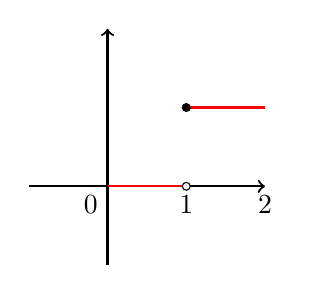
\begin{tikzpicture}
		\draw[->, thick] (-1, 0) -- (2, 0);
		\draw[->, thick] (0, -1) -- (0, 2);
		\draw[red, thick] (0, 0) -- (1, 0);
		\draw[red, thick] (1, 1) -- (2, 1);
		\draw[fill=white] (1, 0) circle (0.05);
		\draw[fill=black] (1, 1) circle (0.05);
		\foreach \x in {1, 2} 
			\node at (\x, 0) [below] {\x};
		\node at (0, 0) [below left] {0};
\end{tikzpicture}
\end{wrapfigure}
Fonctions discontinues:
$x \mapsto [x]$ n'est pas continue en 1 par exemple. En effet, $\displaystyle \lim_{\substack{x\to 1 \\ x<1}} f(x) = 0 \text{et} \lim_{\substack{x\to 1 \\  x>1}} f(x) = 1$.~\\
Les limites à gauches et à droite étant différentes donc $\lim_{x\to 1} \text{ n'existe pas }$


\begin{wrapfigure}{l}{0pt}
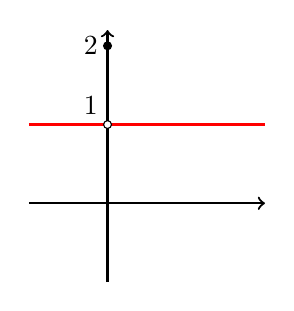
\begin{tikzpicture}
		\draw[->, thick] (-1, 0) -- (2, 0);
		\draw[->, thick] (0, -1) -- (0, 2.2);
		\draw[red, thick] (-1, 1) -- (2, 1);
		\draw[fill=white] (0, 1) circle (0.05) node [above left] {1};
		\draw[fill=black] (0, 2) circle (0.05) node [left] {2};
\end{tikzpicture}
\end{wrapfigure}
$g(x) = 1$ pour tout x différent de 0
mais $\lim_{\substack{x\to 0 \\  x > 0}} g(x) = \lim_{x \to 0; x <0} g(x) $

\paragraph{Remarque} f continue en $x_0$ si et seulement si $\forall \epsilon > 0,$ il existe $\delta >0$ tel que $|x-x_0| < \delta$ et $|f(x) - f(x_0)| < \epsilon$

\paragraph{Définition} \begin{itemize}
\item f est continue à droite en $x_0$ si limite de f(x) par valeur supérieur (\begin{math} \lim_{\substack{x \to x_0 \\ x > x_0}} f(x) \end{math}) en $x_0$ et vaut $f(x_0)$
\item f est continue à gauche e en $x_0$ si limite de f(x) par valeur inférieur (\begin{math} \lim_{\substack{x \to x_0 \\ x < x_0}} f(x) \end{math}) en $x_0$ et vaut $f(x_0)$
\end{itemize}

\paragraph{Exemple} \begin{itemize}
	\item f(partie entière de l'exemple précédent) est continue à droite mais pas à gauche en 1. f est continue sur $[0; 1[$
	\item g n'est pas continue \ul{ni} à gauche, \ul{ni} à droite en 0.
\end{itemize}

\paragraph{Proposition} f est continue en $x_0$ si et seulement si elle est continue à gauche \ul{et} à droite en $x_0$
\paragraph{Propriété} $f, g : E \rightarrow \mathbb{R}, x_0 \in E$ ~\\
f et g continue en $x_0$ 

\begin{itemize}
	\item f+g est continue en $x_0$
	\item f.g est continue en $x_0$
	\item $\frac{f}{g} $est continue en $x_0$ si $g(x_0) \neq 0$
\end{itemize}
La continuité est très local, meme si pour un $x \in E$, $g(x) = 0$, temps que $x_0$ différent de 0, $\frac{f}{g}$ est continue en $x_0$

\paragraph{Composition} $f:E \rightarrow F$ $g:F \rightarrow G$ et $gof : E \rightarrow G$
si f est continue en $x \in E$ et g est continue en $f(x) \in F$, alors gof est continue en $x_0$

\paragraph{Exemple} \begin{itemize}
	\item Polynôme , $\sin+\cos, \tan + exp$ sont continues sur $\mathbb{R}$
	\item $\sin(ln(\frac{e^x}{1+x^2}))$ est continue sur $\mathbb{R}$ car $exp, 1+x^2$ sont continue, de plus $1+x^2 \neq 0$ pour $x \in \mathbb{R}$ donc $\frac{e^x}{1+x^2}$ est continue sur $\mathbb{R}$.
	Finallement, $e^x$ n'est jamais null donc $im(x\mapsto \frac{e^x}{1+x^2}) = \varphi \subset \mathbb{R}^{+*}$, d'où $ln(\varphi)$ est continue sur $\mathbb{R}$

\item $\begin{array}{l}
	x\mapsto \frac{\sin(x)}{x} \\
	\mathbb{R^*} \rightarrow \mathbb{R}
\end{array}$
	 est continue sur $\mathbb{R}^*$, de plus, $\lim_{x \to 0} \frac{\sin(x)}{x} = 1$ 
\end{itemize}

\paragraph{Définition} Soit $f:E \rightarrow \mathbb{R}$, \fbox{$x_0$ adhérent à E}.
Si $\lim_{x\to x_0} f(x) = l$, alors la fonction $g:E\cup \{x_0\} \rightarrow \mathbb{R}$ par la fonction
	\[g(x) = \left\{
			\begin{array}{rl}
				f(x)& \text{ si } x \in  E \\
				l&\text{ si } x = x_0
			\end{array}
			\right. \text{Est continue sur} \mathbb{R}
		\]

\paragraph{Exemple} 

\[g(x) =
	\left\{
			\begin{array}{rl}
				\frac{sin(x)}{x} & \text{ si } x \neq 0 \\
				l&\text{ si } x = 0
			\end{array}
			\right. \text{Est continue sur} \mathbb{R}
		\]

\[h(x) =
	\left\{
			\begin{array}{rl}
				xln(x) & \text{ si } x > 0 \\
				0&\text{ si } x = 0
			\end{array}
			\right. \text { est le prolongement par continuité en 0 de } x\mapsto xln(x)
		\]

		\[x \mapsto \frac{1}{x} \text{ , } \lim_{x \to 0^-} \frac{1}{x} = -\infty \text{ et }
			\lim_{x \to 0^+} \frac{1}{x} = +\infty \]

\paragraph{Exercice} Par quelles valeurs de c, la fonction définie par 
\[f(x) =
	\left\{
			\begin{array}{rl}
				\frac{sin(2x)}{x} & \text{ si } x < 0 \\
				x+c&\text{ si } x \geq 0
			\end{array}
			\right.
		\]

		est continue ? f est continue si et seulement si $x=2$ En effet, \begin{align*} 
		\lim_{\substack{x\to 0 \\ x < 0}} f(x) &= \lim_{\substack{x\to 0 \\ x <0}} \frac{sin(2x)}{x} \\
									  &= \frac{sin(2x)}{2x} * 2 = 2
		\end{align*}

		($2^{eme}$ méthode : $sin(2x) = 2sin(x)*cos(x), \frac{sin(2x)}{x} = 2*\frac{sin(x)}{x}.\cos(x)$ ce qui tend vers 2 pour x tend vers 0, et $\lim_{\substack{x\to 0 \\  x > 0}} f(x) = c$ donc ~\\
		$\lim_{\substack{x\to 0 \\  x > 0}} f(x) = \lim_{\substack{x\to 0 \\  x<0}} f(x) \text{ si et seulement si } c =2$)
		~\\
		Donc f est continue en 0 si $c=0$. De plus, pour tout $x_0 > 0$, $f(x) = x+c$ qui est continue sur $\mathbb{R}^{+*}$ et pour tout $x_0 < 0$, $f(x) = \frac{sin(2x)}{x}$ qui est continue sur $\mathbb{R}^{-*}$
		Le seule problème possible était en 0.

\paragraph{Comportement local}
\paragraph{Proposition} Si f est continue en $x_0$, alors f est localement bornée autour de $x_0$ (c'est à dire il existe un voisinnage de $x_0$ sur lequel f est bornée, c'est à dire il existe $\delta > 0$ et $M > 0$ tel que $|x-x_0| < \delta$ et $|f(x)| < M$).
Si f est continue en $x_0$ et $f(x) \neq 0$, alors f est de signe constant (celui de $f(x_0$) localement autour de $x_0$

\section{Théorème des valeurs intermédiaires}


\begin{wrapfigure}{r}{0cm}
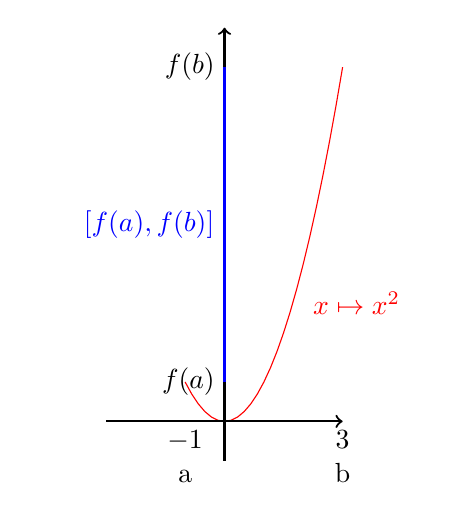
\begin{tikzpicture}[scale=0.5]
	\clip (5, 10) rectangle (-5, -2);
	\draw[domain=-1:3, red] plot(\x, {\x * \x});
	\node at (2, 3) [red, right] {$x \mapsto x^2$};
	\node at (-1, 0) [below, align=center] {$-1$ \\ 
	a};
	\node at (3, 0) [below, align=center] {$3$ \\
	b};
	\draw[->, thick] (-3, 0) -- (3, 0);
	\draw[->, thick] (0, -1) -- (0, 10);
	\node at (0, 1) [left] {$f(a)$};
	\node at (0, 9) [left] {$f(b)$};

	\draw[blue, thick] (0, 1) -- (0, 9) node [left, midway] {$[f(a), f(b)]$};
\end{tikzpicture}
\end{wrapfigure}
\paragraph{Théorème} $f:[a, b] \mathbb{R} (a < b)$ et continue (sur $[a, b]$)
Pour tout y compris entre f(a) et f(b) il existe au moins $x\in [a, b]$ tel que $f(x) = y$.
\paragraph{Exemple} \begin{align*}
	x \mapsto x^2\\
	[-1, 3] \rightarrow \mathbb{R}
\end{align*}

\newpage
\paragraph{(Contre) exemple} : la continuité est essentielle. 
~\\
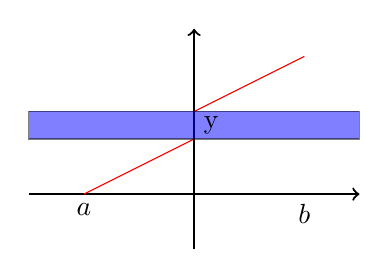
\begin{tikzpicture}[scale=0.7]
	\draw[thick, ->] (-3, 0) -- (3, 0);
	\draw[thick, ->] (0, -1) -- (0, 3);
	\draw[red] (-2, 0) -- (0, 1);
	\draw[red] (0, 1.5) -- (2, 2.5);
	\draw[fill = blue, opacity=0.5] (-3, 1) rectangle (3, 1.5);
	\node at (0, 1.25) [right] {y};
	\node at (-2, 0) [below] {$a$};
	\node at (2, 0) [below] {$b$};
\end{tikzpicture}
~\\
Fonction monotone et non continue pour laquel il existe des y dans $[f(a), f(b)]$ qui n'a pas d'ancédent entre a et b.

~\\

\paragraph{Corollaire 1} $f:[a, b] \rightarrow \mathbb{R}$, continue. ~\\
si f(a) et f(b) sont non nul et de signes différents, il existe $x \in ]a, b[$ tel que $f(x) = 0$
